\documentclass[10pt,a4paper]{article}
\usepackage[utf8]{inputenc}
\usepackage{amsmath}
\usepackage{amsfonts}
\usepackage{amssymb}
\usepackage{graphicx}
\begin{document}
\textbf{Compte rendu de la réunion du 25 mars 2016.}\\\\
Personnes présentes : Mr. Boigelot, Valentin, Julie, Christophe et Hubert.\\\\
Conclusions :
\begin{itemize}
\item Vérifier que le 3è servo du pied est légal
\item Vérifier que le mouvement de bras à 180 degrés autour de l'épaule est légal
\item Peut-on plier les genous dans l'autre sens (robot humanoide ? )
\item Etudier la possibilité d'avoir des pièces absorpantes de chocs dans le robot (pour éviter d'endommager les servos en cas de chocs).
\item Il a été décidé de changer l'agencement des pieds, pour se rapprocher de la solution qui semble être utilisée par la plupart des robots. (comme par Darwin-op, image en dessous)
\begin{figure}[htp]
\center
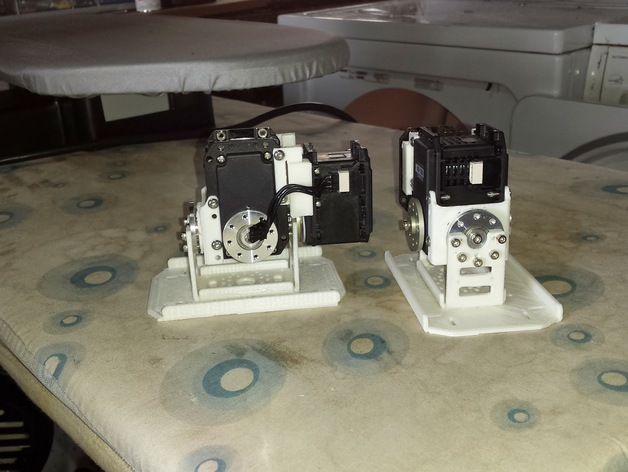
\includegraphics[width=0.7\textwidth]{feet}
\caption{Feet of darwin-op}
\label{feet}
\end{figure}
\end{itemize}
\end{document}